\documentclass[oneside, mag]{mgr}	
 
\usepackage{polski}	
\usepackage[utf8]{inputenc}	
\usepackage{amsmath}		
\usepackage{graphicx}	
\graphicspath{ {./} }
\usepackage{amsfonts}
\usepackage{hyperref}
\usepackage{tabstackengine}
\usepackage{caption}
\usepackage{subfig}
\usepackage{listings}

\newcommand{\bb}{\textbf}

\title{Analiza efektywności zastosowania sieci rekurencyjnych w zadaniu klasyfikacji}	
\engtitle{Analysis of the effectiveness of recursive networks in the classification task}
\author{Jędrzej Kozal}
\supervisor{dr  inż. Paweł Ksieniewicz}

\field{Informatyka (Inf)}
\specialisation{Systemy informatyki w medycynie (IMT)}

\begin{document}
\bibliographystyle{plabbrv}	

\maketitle

\chapter{Wstęp}

\section{Wprowadzenie}

\subsection{Rekurencyjne sieci neuronowe}

Sieci Rekurencyjne zostały oparte na pracy Rumelharta \cite{RNN}. Algorytm uczenia RNN - propagacja wsteczna w czasie (Back-Propagation Through Time - BPTT) zostały przedstawione w \cite{BPTT}.
Udowodniono, że przy pewnych założeniach RNN są kompletne w sensie Turinga \cite{turing-complete}.

\subsection{Zastosowania rekurencyjnych sieci neuronowych}

Sieci Rekurencyjne znalazły wiele zastosowań w przetwarzaniu sekwencji. (opisać zastosowania) NLP: tłumaczenie, modele języka, naśladowanie stylu, przetwarzanie dźwięków: generowanie mowy, generowanie muzyki, sentiment analysis 

Sieci rekurencyjne są także wykorzystywane w połączeniu z innymi modelami jak np. labelowanie images.

\subsection{Zadanie klasyfikacji}

\cite{Goodfellow-et-al-2016}

\section{Przegląd literatury}

Wprowadzono wiele modyfikacji w zakresie zasad działania i strukturze RNN. 
W \cite{bidirectional} wprowadzono sieci dwukierunkowe, przetwarzające sekwencje w dwóch kierunkach: od początku do końca sekwencji i od końca do początku. Ostateczna wartość dla n-tego elementu sekwencji jest obliczana na podstawie n-tego wyniku dla obu kierunków.

RNN w swojej natywnej formie nie są w stanie nauczyć się długich zależności w ciągu uczącym. Problem ten jest w znacznej mierze spowodowany wybuchającymi lub znikającymi gradientami (exploding or vanishing gradients \cite{vanishing_gradient_RNN}). W celu zaadresowania tego problemu Hochreiter i Schmidhuber zaproponowali architekturę Long Short-Term Memory (LSTM) \cite{LSTM}. LSTM oprócz wewnętrznego stanu sieci posiada także komórkę pamięci, w której może przechowywać informacje przez długi czas. Bramki to dodatkowe elementy pozwalające na regulowanie aktualnych wartości zmiennych sieci. Ponieważ bramka to warstwa sieci z sigmoidalną funkcją aktywacji (sigmoidalna funkcja aktywacji posiada zakres wartości $(0,1)$) to sieć może się nauczyć w którym momencie i w jaki sposób uaktualniać swoją komórkę pamięci i swój wewnętrzny stan. Trzy bramki stosowane przez LSTM to forget gate, input gate, oraz output gate.  

Gated Recurrent Unit (GRU) \cite{DBLP:journals/corr/ChungGCB15} jest modyfikacją LSTM. Podstawowa zasada działania modelu zostaje taka sama. Wprowadzone zmiany dotyczą struktury sieci i polegają na zastosowaniu dwóch zamiast trzech komórek, co powoduje zmniejszenie liczby parametrów. Mniejsza liczba parametrów przekłada się na zmniejszenie wymagań w zakresie mocy obliczeniowej potrzebnych do nauczenia modelu, co może mieć przełożenie na zwiększenie głębokości modelu lub zwiększenie ukrytych jednostek. Z drugiej strony zmniejszenie liczby bramek powoduje zmniejszenie mocy modelu. Z praktycznego punktu widzenia LSTM i GRU uzyskują porównywalne wyniki \cite{DBLP:journals/corr/ChungGCB14}.

Rozwinięciem idei wykorzystania pamięci do usprawnienia działania sieci są Neuronowe Maszyny Turinga \cite{DBLP:journals/corr/GravesWD14}. Neuronowe Maszyny Turinga korzystają z mechanizmu uwagi do operacji na pamięci. Pamięć przypomina pamięć dostępną w komputerze i składa się z wielu wektorów, które można wykorzystać do odczytu lub przechowywania informacji. Neuronowa Maszyna Turinga posiada dwie głowice: do zapisu i odczytu. Adresowanie pamięci odbywa się na podstawie zawartości (content-base addressing) lub położenia (location-base addressing).

W \cite{DBLP:journals/corr/VisinKCMCB15} wykorzystano sieć rekurencyjną do klasyfikacji obrazów i porównano uzyskane wyniki z rezultatami dla sieci konwolucyjnych. Proponowany model (ReNet) wykorzystywał RNN do czterotnego trawersowania fragmentów obrazu w celu ekstrakcji cech, jako alternatywę dla warstw konwolucyjnych z poolingiem. W \cite{DBLP:journals/corr/KalchbrennerDG15} przedstawiono GRID LSTM, które rozszerzało standardowy model sieci LSTM do N-wymiarowych komórek ze współdzielonymi wektorami stanu i pamięci.

\chapter{Omówienie wybranych zagadnień teoretycznych}

W tym rozdziale zostały omówione teoretyczne podstawy wybranych algorytmów i struktur sieci, które zostały wykorzystane w badaniach.

\section{Rekurencyjna Sieć Neuronowa}

\section{Propagacja wsteczna w czasie}

\section{LSTM}

\begin{figure}
\centering
	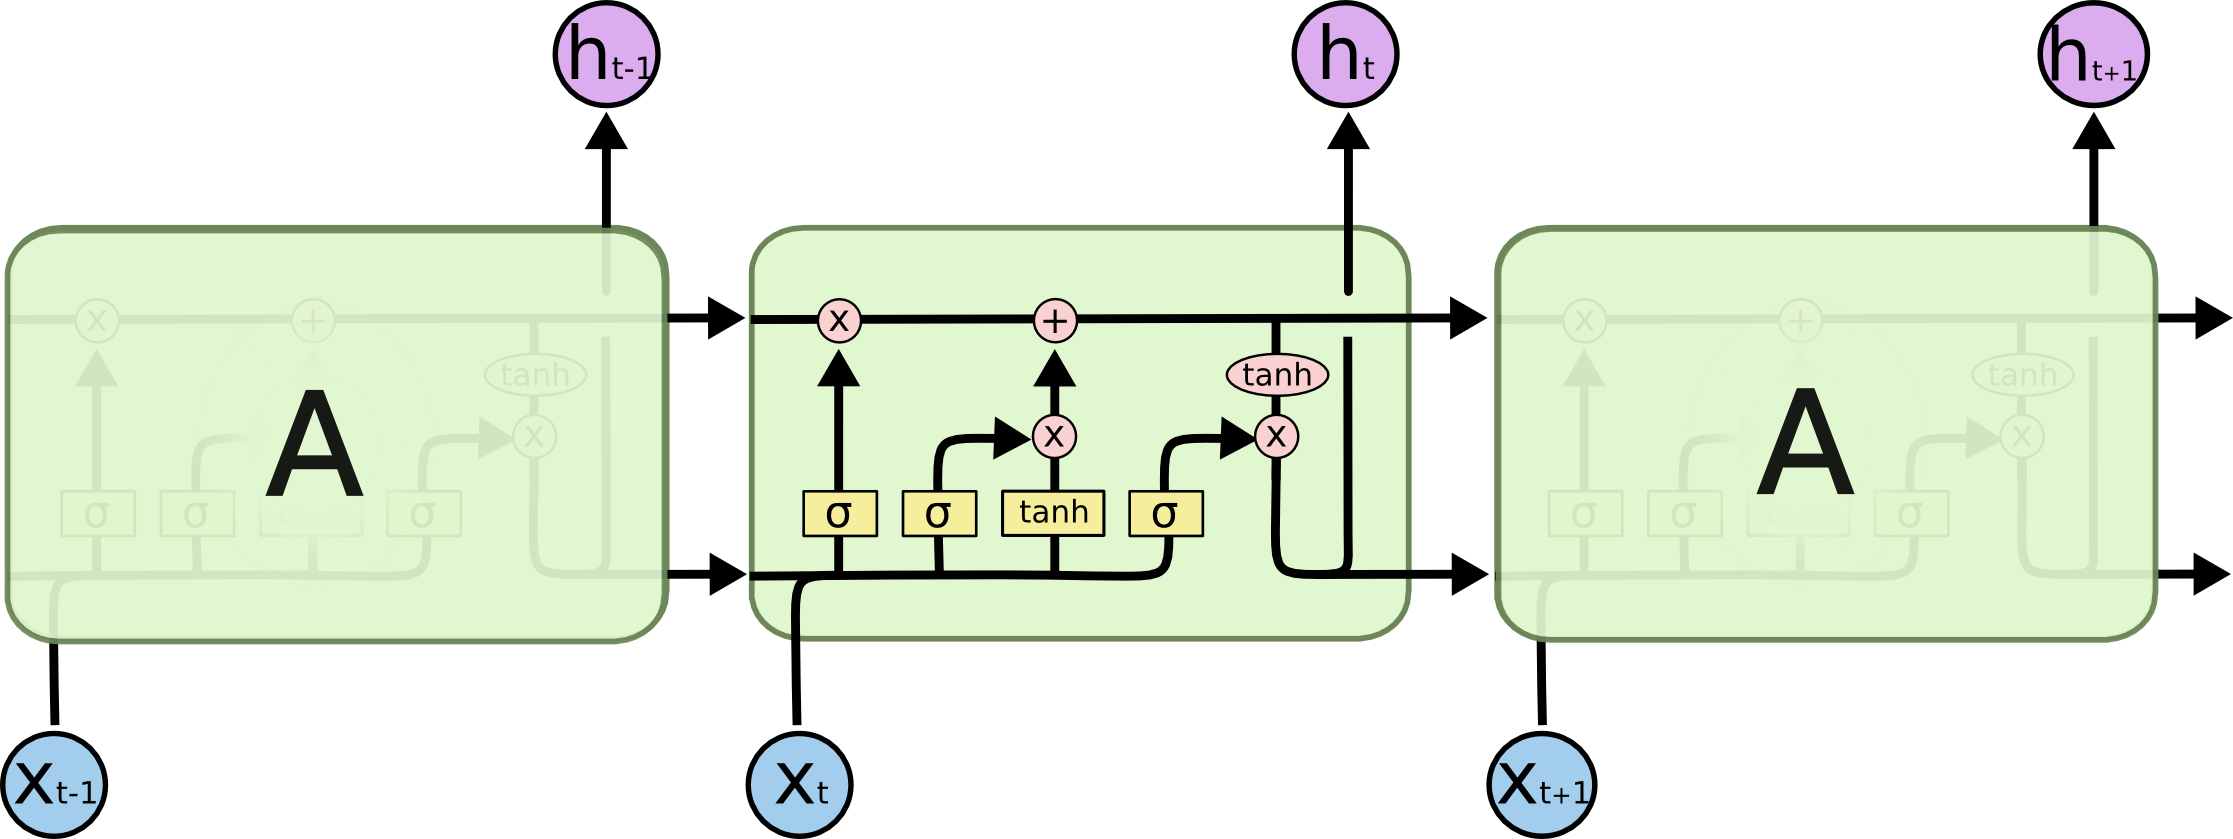
\includegraphics[width=0.90\textwidth]{img/lstm_colah.png}
	\caption{Schemat komórki LSTM.\\ Źródło: http://colah.github.io/posts/2015-08-Understanding-LSTMs/}
	\label{fig:lstm}
\end{figure}

\begin{equation}
\centering
\begin{split}
	f_t = \sigma( W_f [ h_{t-1}, x_t ] + b_f ) \\
	i_t = \sigma( W_i [ h_{t-1}, x_t ] + b_i ) \\
	\tilde{C}_t = tanh( W_c [ h_{t-1}, x_t ] + b_C ) \\
	C_t = f_t * C_{t-1} + i_t * \tilde{C}_t \\
	o_t = \sigma( W_o [ h_{t-1}, x_t ] + b_o ) \\
	h_t = o_t * tanh( C_t )
\end{split}
\end{equation}


\section{GRU}

\begin{figure}
\centering
	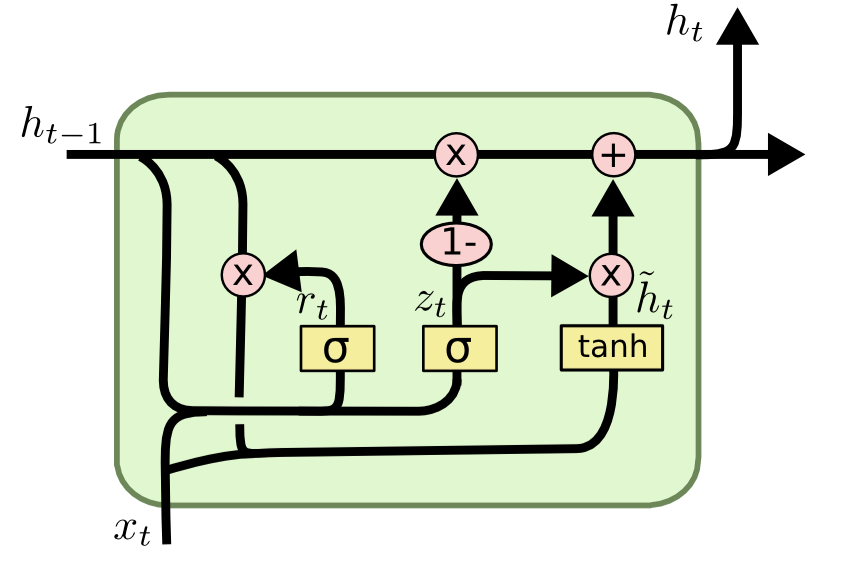
\includegraphics[width=0.5\textwidth]{img/LSTM3-var-GRU.png}
	\caption{Schemat komórki GRU.\\ Źródło: http://colah.github.io/posts/2015-08-Understanding-LSTMs/}
	\label{fig:gru}
\end{figure}

\chapter{Przyjęta metodyka badań}


\section{Problem badawczy}


\section{Opis eksperymentu}

\subsection{Zbiór danych}

\subsection{Wykorzystane narzędzia i hardware}

\subsection{Dobór hiperparametrów modelu}


\chapter{Wyniki}


\chapter{Wnioski}

\bibliography{bibliography}

\tableofcontents

\listoffigures

\end{document}